\documentclass[12pt]{article}
\usepackage{geometry}
%\usepackage{times}
\geometry{a4paper, left=1in, right=1in, bottom=1in, top=1in}
\usepackage{authblk}
\usepackage{fancyhdr}
\usepackage{graphicx}
\usepackage{tabularx}
\usepackage{colortbl}
\usepackage{tabularx}

%define vars
\newcommand{\tit}{Intall Abaqus 2017 on a Linux System}
\newcommand{\ifp}{\textit{InstallationFilesFolder}}
\newcommand{\cmd}[1]{
    \leavevmode{\parindent=0.05\textwidth\indent
    \begin{tabular}{>{\columncolor[gray]{0.8}}p{0.95\textwidth}}
        #1
    \end{tabular}
    }
}

%Paragraph
\setlength{\parindent}{0pt}
\renewcommand{\baselinestretch}{1.3}

%Title page
\title{
\includegraphics[height=1in]{Figures/NUIG_Logo.jpg}\\ \tit}
\author[1]{Yadong Jiang}
\affil[1]{College of Engineering and Informatics, National University of Ireland Galway}
\date{}

%Header and footer
\pagestyle{fancy}
\fancyhf{}
\lhead{
\includegraphics[height=0.5in]{Figures/NUIG_Logo.jpg}}
%\rhead{Yadong Jiang}
\rhead{\tit}
\setlength{\headsep}{0.5in}
\rfoot{Page \thepage}

%Tabular
\def\arraystretch{1.5}

\begin{document}
\maketitle

\newpage

\section*{Description}
This document aims to guide users to install and run Abaqus 2017 on a Linux machine. Table \ref{tb-1} summarizes the installation environments used in this guidance. Although Ubuntu is specified in the table, this instruction file is also suitable for installation of Abaqus on other Linux distributions (e.g. Archlinux, Fedora, etc.). The Linux desktop environment is not required. All installation steps are completed in terminal. Thus, this document is also suitable for users who want to install and run Abaqus on a Linux server remotely via SSH connection. But it should be highlighted that the administration right is required to complete the installation.

\begin{table}[h!]
\caption{Environments of Installation}
\begin{center}
\begin{tabular}{l l}
    \hline
    Linux Distribution: & Ubuntu 14.04.4 LTS (64 bits)\\
    \hline
    Linux desktop environment: & N/A \\
    \hline
    Administration Right: & Yes \\
    \hline
    Abaqus version: & Abaqus 2017 (64 bits) \\
    \hline
\end{tabular}
\end{center}
\label{tb-1}
\end{table}

\section*{Prerequirments}

\cmd{sudo apt-get install ksh lsb-core}


\subsection*{Install Required Packages}

\subsection*{Disguise Your Linux Distribution}
\begin{figure}[h!]
\label{fig-1}
\begin{center}
    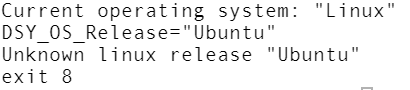
\includegraphics[width=0.5\textwidth]{Figures/UnknowLinux.png}
\end{center}
\caption{Unknown linux release}
\end{figure}


\begin{table}[h!]
\label{tb-2}
\caption{Folders which contain the ``Linux.sh`` files}
\begin{center}
\begin{tabular}{l}
    \hline
    \ifp/1/inst/common/init \\
    \hline
    \ifp/1/SIMULIA\_Documentation/AllOS/1/inst/common/init \\
    \hline
    \ifp/2/SIMULIA\_FLEXnet\_LicenseServer/Linux64/1/inst/common/init \\
    \hline
    \ifp/2/SIMULIA\_AbaqusServices/Linux64/1/inst/common/init \\
    \hline
    \ifp/2/SIMULIA\_AbaqusServices\_CAA\_API/Linux64/1/inst/common/init \\
    \hline
    \ifp/2/SIMULIA\_Abaqus\_CAE/Linux64/1/inst/common/init \\
    \hline
    \ifp/2/SIMULIA\_Tosca/Linux64/1/inst/common/init \\
    \hline
    \ifp/3/SIMULIA\_Isight/Linux64/1/inst/common/init \\
    \hline
\end{tabular}
\end{center}
\end{table}

\begin{figure}[h!]
\label{fig-2}
\begin{center}
    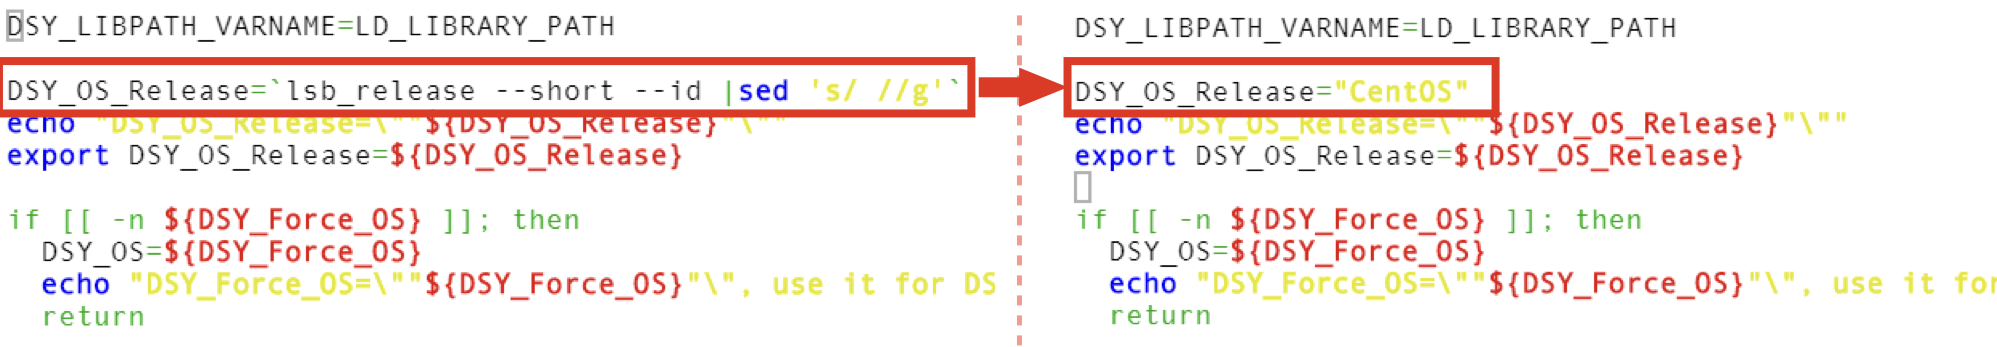
\includegraphics[width=\textwidth]{Figures/FakeLinux.png}
\end{center}
\caption{Change the ``Linux.sh`` file}
\end{figure}



\section*{Installation}

\begin{figure}[h!]
    \label{fig-3}
    \begin{center}
        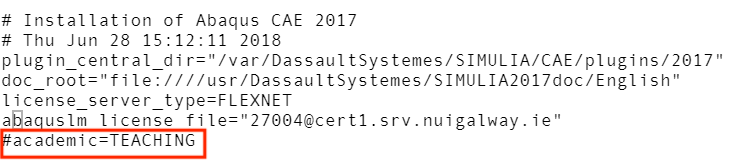
\includegraphics[width=\textwidth]{Figures/Custom_v6.png}
    \end{center}
    \caption{Change the license setting in the ``custom\_v6.env`` file}
\end{figure}

\section*{Start Abaqus}

\end{document}